\cleardoublepage

\chapter{Porównawcza analiza wydajności REST i~gRPC-Web}
\label{cha:AnalizaWydajnosci}

Wyniki eksperymentu przeprowadzonego zgodnie z~metodologią z~rozdziału~\ref{cha:MetodologiaBadan} układają się w~jeden wątek wyjaśniający: różnica pomiędzy protokołami pojawia się wtedy, gdy mniejszy ładunek pozwala przesłać odpowiedź w~mniejszej liczbie etapów transmisji. Analiza prowadzi od~zmierzonego wolumenu danych i~modelu liczby wymian pakietów, przez trzy grupy scenariuszy oraz ocenę niepewności, do~weryfikacji hipotez, zestawienia z~dotychczasowymi badaniami i~wytycznych wdrożeniowych.

% -----------------------------------------------------------------------
\section{Wolumen przesyłanych danych}
\label{sec:WolumenDanych}
% -----------------------------------------------------------------------

Rozmiary odpowiedzi wyznaczono pomiarowo na~wdrożonym systemie, zestawiając liczbę bajtów zwracanych przez punkt końcowy REST oraz przez usługę gRPC dla identycznego zapytania. Wyniki przedstawia tabela~\ref{tab:WolumenDanych}.

\begin{table}[htb]
\centering
\footnotesize
\caption{Zmierzony rozmiar odpowiedzi [B] i~redukcja uzyskana serializacją binarną}
\label{tab:WolumenDanych}
\begin{tabular}{|l|c|r|r|c|}
\hline
\textbf{Scenariusz} & \textbf{Rekordów} & \textbf{JSON} & \textbf{Protocol Buffers} & \textbf{Redukcja} \\
\hline
Products & 10   & 1\,328   & 752      & 43,4\% \\
Products & 200  & 26\,405  & 14\,998  & 43,2\% \\
Products & 500  & 66\,556  & 38\,054  & 42,8\% \\
Products & 1000 & 133\,134 & 76\,200$^{*}$  & 42,8\%$^{*}$ \\
Products & 2000 & 265\,159 & 151\,700$^{*}$ & 42,8\%$^{*}$ \\
\hline
Echo     & 10   & 1\,771   & 1\,190   & 32,8\% \\
Echo     & 200  & 36\,242  & 24\,104  & 33,5\% \\
\hline
\multicolumn{5}{|l|}{\footnotesize $^{*}$ wartość oszacowana przez ekstrapolację zmierzonego współczynnika redukcji} \\
\hline
\end{tabular}
\end{table}

Serializacja binarna redukuje wolumen przesyłanych danych o~42,8--43,4\% w~scenariuszu Products oraz o~32,8--33,5\% w~scenariuszu Echo. Stabilność współczynnika względem liczby rekordów potwierdza jego systematyczny charakter.

\subsection{Wpływ kompresji treści na~wolumen danych}
\label{subsec:Kompresja}

Wszystkie rozmiary przedstawione w~tabeli~\ref{tab:WolumenDanych} dotyczą treści nieskompresowanej. W~badanym systemie kompresja ciała odpowiedzi nie została włączona na~żadnej ze~ścieżek: usługi nie korzystają z~oprogramowania pośredniczącego kompresji, a~konfiguracja serwera pośredniczącego nie zawiera filtra kompresora. Dla wszystkich badanych wariantów zastosowano tę~samą politykę braku kompresji. Podejście to~odpowiada domyślnym ustawieniom platformy ASP.NET Core oraz szkieletu gRPC dla~.NET. Ponieważ JSON i~Protocol Buffers różnią się podatnością na~kompresję, konsekwencje tego wyboru dla zakresu wniosków wymagają jednak omówienia; w~praktyce wdrożeniowej dokumenty JSON podawane są~najczęściej z~kompresją realizowaną przez serwer aplikacyjny, odwrotne proxy lub sieć dostarczania treści.

Wpływ kompresji oszacowano ilościowo dla scenariusza Echo, którego ładunek generowany jest w~sposób deterministyczny. Poprawność odtworzenia zweryfikowano przez porównanie z~rozmiarami zmierzonymi na~wdrożonym systemie: dla 200~rekordów uzyskano 36\,246~B wobec zmierzonych 36\,242~B w~formacie JSON oraz 24\,079~B wobec 24\,104~B w~formacie binarnym, czyli odchylenie nieprzekraczające 0,1\%. Wyniki kompresji algorytmem gzip przedstawia tabela~\ref{tab:Kompresja}.

\begin{table}[htb]
\centering
\footnotesize
\caption{Rozmiar ładunku scenariusza Echo bez~kompresji i~po~kompresji gzip [B] oraz stosunek rozmiaru do~efektywnego progu transmisji}
\label{tab:Kompresja}
\begin{tabular}{|c|r|r|r|r|c|c|}
\hline
\textbf{Rek.} & \textbf{JSON} & \textbf{JSON gz} & \textbf{protobuf} & \textbf{protobuf gz} & \textbf{$s/W_{\mathrm{eff}}$ JSON gz} & \textbf{$s/W_{\mathrm{eff}}$ protobuf} \\
\hline
200  & 36\,246  & 2\,964  & 24\,079  & 2\,523  & 0,05 & 0,37 \\
500  & 91\,247  & 7\,129  & 60\,679  & 5\,986  & 0,11 & 0,93 \\
2000 & 370\,255 & 27\,715 & 246\,682 & 22\,686 & 0,42 & 3,76 \\
\hline
\end{tabular}
\end{table}

Dwie ostatnie kolumny przedstawiają stosunek rozmiaru odpowiedzi do~zaobserwowanego efektywnego progu transmisji dla konfiguracji spotykanych w~praktyce wdrożeniowej: dokumentu JSON podawanego z~kompresją oraz komunikatu binarnego przesyłanego bez~niej, ponieważ kompresja gRPC bywa włączana rzadziej. Kompresja redukuje wolumen formatu tekstowego 12--13-krotnie, a~formatu binarnego 9,5--11-krotnie. Po~jej zastosowaniu przewaga objętościowa serializacji binarnej maleje z~33\% do~15--18\%. Wszystkie badane ładunki pozostają wówczas poniżej efektywnego progu transmisji. Przeniesienie wyników dla transferów nieskompresowanych na~wdrożenie z~włączoną kompresją wymagałoby odrębnego pomiaru.

% -----------------------------------------------------------------------
\section{Model liczby wymian pakietów}
\label{sec:ModelOkna}
% -----------------------------------------------------------------------

Zmierzona charakterystyka łącza ujawniła, że~przepustowość pojedynczego połączenia wynosi około 20~Mbit/s, mimo że~przepustowość zagregowana przekracza 270~Mbit/s. Iloczyn przepustowości i~opóźnienia dla tego połączenia wynosi

\begin{equation}
20~\mathrm{Mbit/s} \cdot 0{,}0262~\mathrm{s} \approx 65\,500~\mathrm{B} \approx 64~\mathrm{KiB},
\label{eq:BDP}
\end{equation}

co~odpowiada rozmiarowi okna odbiorczego protokołu TCP bez~zastosowania skalowania okna~\cite{bib:RFC9293}. Wartość tę~przyjęto dalej jako zaobserwowany efektywny próg transmisji, bez rozstrzygania, który mechanizm TCP go~wyznacza. Przy oknie mniejszym od~iloczynu przepustowości i~opóźnienia przepustowość osiągalna w~jednym połączeniu jest wyznaczona rozmiarem okna. Czynnikiem ograniczającym pojedyncze żądanie pozostaje ilość danych, jaką nadawca może wysłać przed otrzymaniem potwierdzenia: po~wypełnieniu okna transmisja wstrzymuje się do~nadejścia potwierdzenia od~odbiorcy.

Zależność $B = W / \mathrm{RTT}$ pozwala oszacować rozmiar okna $W$ na~podstawie zmierzonej przepustowości pojedynczego połączenia $B$ i~opóźnienia obiegu pakietu. Sama zgodność oszacowania z~wartością 64~KiB nie przesądza o~tym, czy~ograniczeniem jest okno odbiorcze, czy~powolny start TCP. Rozróżnienie tych mechanizmów wymagałoby przechwycenia ruchu na~poziomie pakietów, którego nie wykonano. Oba mechanizmy mogą prowadzić do~skokowego wzrostu kosztu transmisji związanego z~koniecznością oczekiwania na~kolejne potwierdzenia.

Na~potrzeby modelu zaobserwowany efektywny próg transmisji oznaczono przez $W_{\mathrm{eff}} \approx 64~\mathrm{KiB}$. Przesłanie odpowiedzi o~rozmiarze $s$ wymaga $\lceil s / W_{\mathrm{eff}} \rceil$ etapów transmisji, a~każdy etap ponad pierwszy kosztuje jedno dodatkowe opóźnienie obiegu pakietu. Przewidywana liczba dodatkowych obiegów wynosi zatem

\begin{equation}
n_{\mathrm{RTT}} = \left\lceil \frac{s}{W_{\mathrm{eff}}} \right\rceil - 1.
\label{eq:WindowModel}
\end{equation}

Model wyrażony równaniem~\ref{eq:WindowModel} poddano weryfikacji ilościowej, przyjmując za~punkt odniesienia konfigurację o~200~rekordach, w~której odpowiedź obu formatów pozostaje poniżej efektywnego progu transmisji. Rozmiary oznaczone gwiazdką wyznaczono przez ekstrapolację zmierzonego rozmiaru pojedynczego rekordu, niezależne oszacowanie tych samych ładunków, uzyskane przez odtworzenie deterministycznej treści scenariusza Echo (tabela~\ref{tab:Kompresja}), różni się od~nich o~mniej niż 2,5\%, co~nie zmienia przewidywanej liczby dodatkowych obiegów. Nadwyżkę czasu względem tego punktu odniesienia podzielono przez zmierzone opóźnienie obiegu pakietu (26,2~ms). Wyniki przedstawia tabela~\ref{tab:WeryfikacjaModelu}.

\begin{table}[htb]
\centering
\footnotesize
\caption{Weryfikacja modelu: przewidywana i~zmierzona liczba dodatkowych obiegów pakietu}
\label{tab:WeryfikacjaModelu}
\begin{tabular}{|l|c|r|c|c|c|}
\hline
\textbf{Scenariusz} & \textbf{Rekordów} & \textbf{Rozmiar [B]} & \textbf{$s/W_{\mathrm{eff}}$} & \textbf{Przewid.} & \textbf{Zmierz.} \\
\hline
Echo, JSON      & 500  & 90\,500$^{*}$   & 1,38 & 1 & 1,04 \\
Echo, JSON      & 2000 & 362\,000$^{*}$  & 5,52 & 5 & 5,15 \\
Echo, protobuf  & 500  & 60\,500$^{*}$   & 0,92 & 0 & 0,10 \\
Echo, protobuf  & 2000 & 242\,000$^{*}$  & 3,69 & 3 & 3,29 \\
\hline
Products, JSON      & 500  & 66\,556   & 1,02 & 1 & 0,97 \\
Products, JSON      & 1000 & 133\,134  & 2,03 & 2 & 1,89 \\
Products, JSON      & 2000 & 265\,159  & 4,05 & 4 & 3,83 \\
Products, protobuf  & 500  & 38\,054   & 0,58 & 0 & 0,08 \\
Products, protobuf  & 1000 & 76\,200$^{*}$   & 1,16 & 1 & 1,06 \\
Products, protobuf  & 2000 & 151\,700$^{*}$  & 2,31 & 2 & 2,19 \\
\hline
\multicolumn{6}{|l|}{\footnotesize $^{*}$ wartość wyznaczona przez ekstrapolację zmierzonego rozmiaru pojedynczego rekordu} \\
\hline
\end{tabular}
\end{table}

Zgodność jest bardzo dobra we~wszystkich dziesięciu przypadkach: różnica pomiędzy wartością przewidywaną a~zmierzoną nie przekracza 0,29~obiegu, a~w~żadnym przypadku nie zmienia liczby całkowitej. Model wyjaśnia w~szczególności zjawisko, którego nie sposób wyjaśnić samą przepustowością: różnica 30~kilobajtów pomiędzy formatami przy 500~rekordach scenariusza Echo odpowiadałaby przy przepustowości zagregowanej niespełna jednej milisekundy, a~przy przepustowości pojedynczego strumienia około dwunastu milisekund. Zmierzona różnica wynosi 26~ms, czyli dokładnie jeden obieg pakietu.

Przewaga serializacji binarnej realizuje się zatem skokowo, gdy odpowiedź przekracza kolejne wielokrotności $W_{\mathrm{eff}}$, i~w~modelu skaluje się z~opóźnieniem obiegu pakietu. Model przewiduje, że~w~sieci lokalnej, gdzie opóźnienie jest mniejsze od~milisekundy, ten~sam mechanizm dawałby korzyść znacznie mniejszą.

% -----------------------------------------------------------------------
\section{Analiza narzutu protokołu (Echo)}
\label{sec:AnalizaEcho}
% -----------------------------------------------------------------------

Scenariusze Echo izolują koszt protokołu od~kosztu warstwy danych. Tabela~\ref{tab:EchoLatency} przedstawia zmierzone mediany opóźnień wraz ze~współczynnikami zmienności. Zależność tę~przedstawia rysunek~\ref{fig:WykresEcho}.

\begin{table}[htb]
\centering
\footnotesize
\caption{Mediana opóźnienia w~scenariuszach Echo [ms]; w~nawiasach współczynnik zmienności median pięciu przebiegów}
\label{tab:EchoLatency}
\begin{tabular}{|c|c|c|c|c|c|}
\hline
\textbf{VU} & \textbf{Rekordów} & \textbf{REST} & \textbf{Envoy} & \textbf{Direct} & \textbf{Direct vs REST} \\
\hline
10 & 10   & 31,0 (0,7\%) & 32,6 (4,6\%) & 30,1 (2,9\%) & $-$3\% \\
10 & 100  & 32,1 (2,9\%) & 32,2 (1,5\%) & 30,8 (3,4\%) & $-$4\% \\
10 & 200  & 32,6 (1,1\%) & 33,3 (1,5\%) & 31,3 (1,3\%) & $-$4\% \\
10 & 500  & 59,8 (1,0\%) & 35,2 (1,8\%) & 33,8 (2,3\%) & $\mathbf{-43\%}$ \\
10 & 2000 & 167,6 (0,7\%) & 120,8 (1,8\%) & 117,4 (1,6\%) & $\mathbf{-30\%}$ \\
\hline
20 & 10   & 37,1 (5,7\%) & 34,8 (4,0\%) & 32,5 (3,6\%) & $-$12\% \\
20 & 100  & 39,0 (4,3\%) & 35,6 (6,9\%) & 33,0 (3,3\%) & $-$15\% \\
20 & 200  & 37,0 (5,6\%) & 34,9 (1,7\%) & 33,8 (3,0\%) & $-$9\% \\
20 & 500  & 60,6 (1,7\%) & 39,1 (6,0\%) & 35,5 (11,5\%) & $\mathbf{-41\%}$ \\
\hline
\end{tabular}
\end{table}

\begin{figure}[htb]
\centering
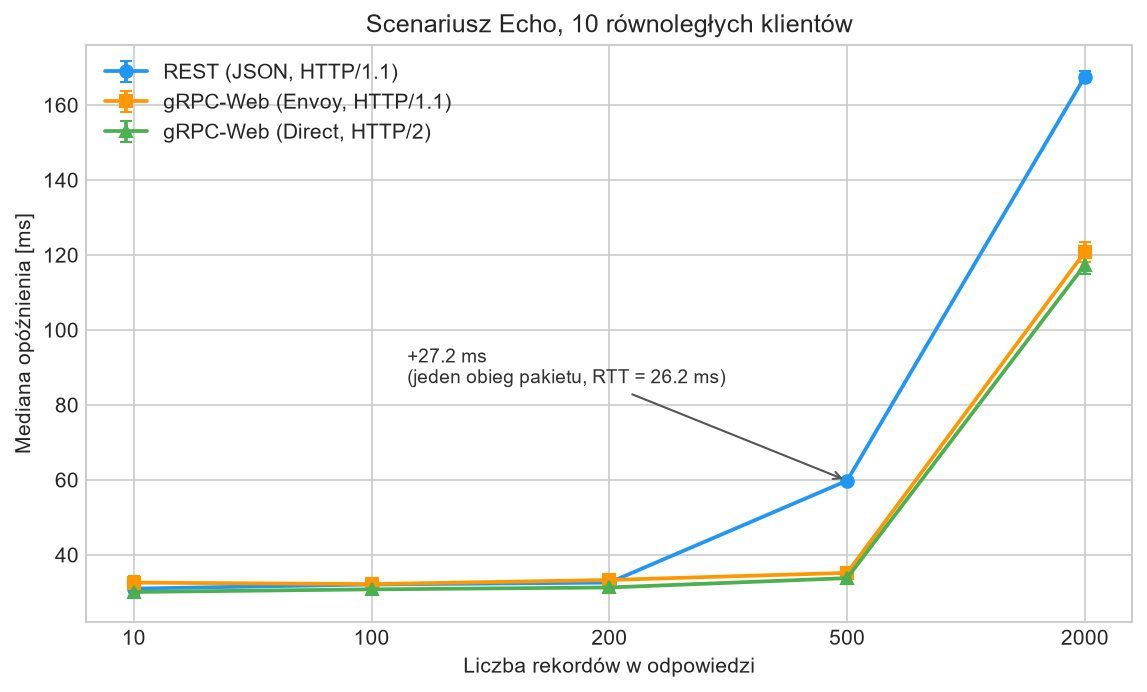
\includegraphics[width=0.7\textwidth]{figures/chart_browser_echo.png}
\caption{Mediana opóźnienia w~scenariuszach Echo względem liczby rekordów w~odpowiedzi}
\label{fig:WykresEcho}
\end{figure}

Do~200~rekordów włącznie różnice pomiędzy protokołami pozostają niewielkie, od~trzech do~piętnastu procent, przy wartościach bezwzględnych rzędu kilku milisekund. Zgodnie z~modelem z~sekcji~\ref{sec:ModelOkna} odpowiedzi tego rozmiaru pozostają poniżej efektywnego progu transmisji w~obu formatach, liczba obiegów pakietu jest zatem identyczna, a~pozostała różnica wynika z~narzutu ramkowania i~warstwy transportowej.

Przejście z~200 na~500~rekordów powoduje skokową zmianę obrazu. Opóźnienie REST rośnie z~32,6 do~59,8~ms, czyli o~27,2~ms. W~tym samym przejściu wariant Direct przechodzi z~31,3 do~33,8~ms, czyli o~2,5~ms. Przewaga wariantu binarnego osiąga w~tej konfiguracji 43\%: dokument JSON o~rozmiarze 90,5~kilobajta przekracza efektywny próg transmisji, a~wiadomość binarna o~rozmiarze 60,5~kilobajta pozostaje poniżej niego.

Przy 2000~rekordach przewaga wynosi 30\%, czyli zbliża się do~zmierzonego współczynnika redukcji wolumenu danych. Przy odpowiedziach przekraczających kilka wielokrotności $W_{\mathrm{eff}}$ liczba obiegów staje się w~przybliżeniu proporcjonalna do~rozmiaru odpowiedzi, a~przewaga czasowa zbiega wówczas do~przewagi objętościowej.

Współczynniki zmienności nie przekraczają w~tej grupie 6,9\%, z~jednym wyjątkiem na~poziomie 11,5\%. Wszystkie omówione relacje zachodzą konsekwentnie w~każdym z~pięciu przebiegów.

% -----------------------------------------------------------------------
\section{Analiza wydajności odczytu (Products)}
\label{sec:AnalizaProducts}
% -----------------------------------------------------------------------

Scenariusze Products badają wydajność w~realistycznym kontekście odczytu katalogu, z~pełnym łańcuchem obejmującym pamięć podręczną lub bazę danych, deserializację w~przeglądarce oraz aktualizację interfejsu.

\subsection{Odczyt z~ciepłą pamięcią podręczną}
\label{subsec:ProductsWarm}

Mediany opóźnienia zmierzone przy buforze wypełnionym przedstawia tabela~\ref{tab:ProductsWarm}.

\begin{table}[htb]
\centering
\footnotesize
\caption{Mediana opóźnienia w~scenariuszach Products, ciepła pamięć podręczna [ms]; w~nawiasach współczynnik zmienności median pięciu przebiegów}
\label{tab:ProductsWarm}
\begin{tabular}{|c|c|c|c|c|c|}
\hline
\textbf{VU} & \textbf{PageSize} & \textbf{REST} & \textbf{Envoy} & \textbf{Direct} & \textbf{Direct vs REST} \\
\hline
10 & 10   & 33,6 (6,7\%) & 34,9 (2,0\%) & 31,7 (2,7\%) & $-$6\% \\
10 & 100  & 39,2 (8,0\%) & 41,7 (6,3\%) & 39,0 (2,6\%) & $-$1\% \\
10 & 200  & 40,3 (3,7\%) & 42,0 (5,7\%) & 39,0 (5,0\%) & $-$3\% \\
10 & 500  & 65,8 (0,6\%) & 42,3 (4,5\%) & 41,1 (3,5\%) & $\mathbf{-38\%}$ \\
10 & 1000 & 89,9 (1,4\%) & 69,4 (4,5\%) & 66,9 (1,0\%) & $\mathbf{-26\%}$ \\
10 & 2000 & 140,6 (1,6\%) & 97,5 (1,8\%) & 96,5 (1,4\%) & $\mathbf{-31\%}$ \\
\hline
20 & 10   & 40,9 (4,6\%) & 37,5 (6,2\%) & 34,4 (1,4\%) & $-$16\% \\
20 & 100  & 45,5 (2,9\%) & 45,2 (3,0\%) & 43,6 (7,2\%) & $-$4\% \\
20 & 200  & 46,2 (3,0\%) & 45,9 (3,0\%) & 44,4 (4,5\%) & $-$4\% \\
20 & 500  & 71,8 (1,5\%) & 48,4 (2,8\%) & 44,4 (3,1\%) & $\mathbf{-38\%}$ \\
20 & 1000 & 94,3 (2,4\%) & 70,5 (1,6\%) & 70,2 (2,2\%) & $\mathbf{-26\%}$ \\
\hline
\end{tabular}
\end{table}

\begin{figure}[htb]
\centering
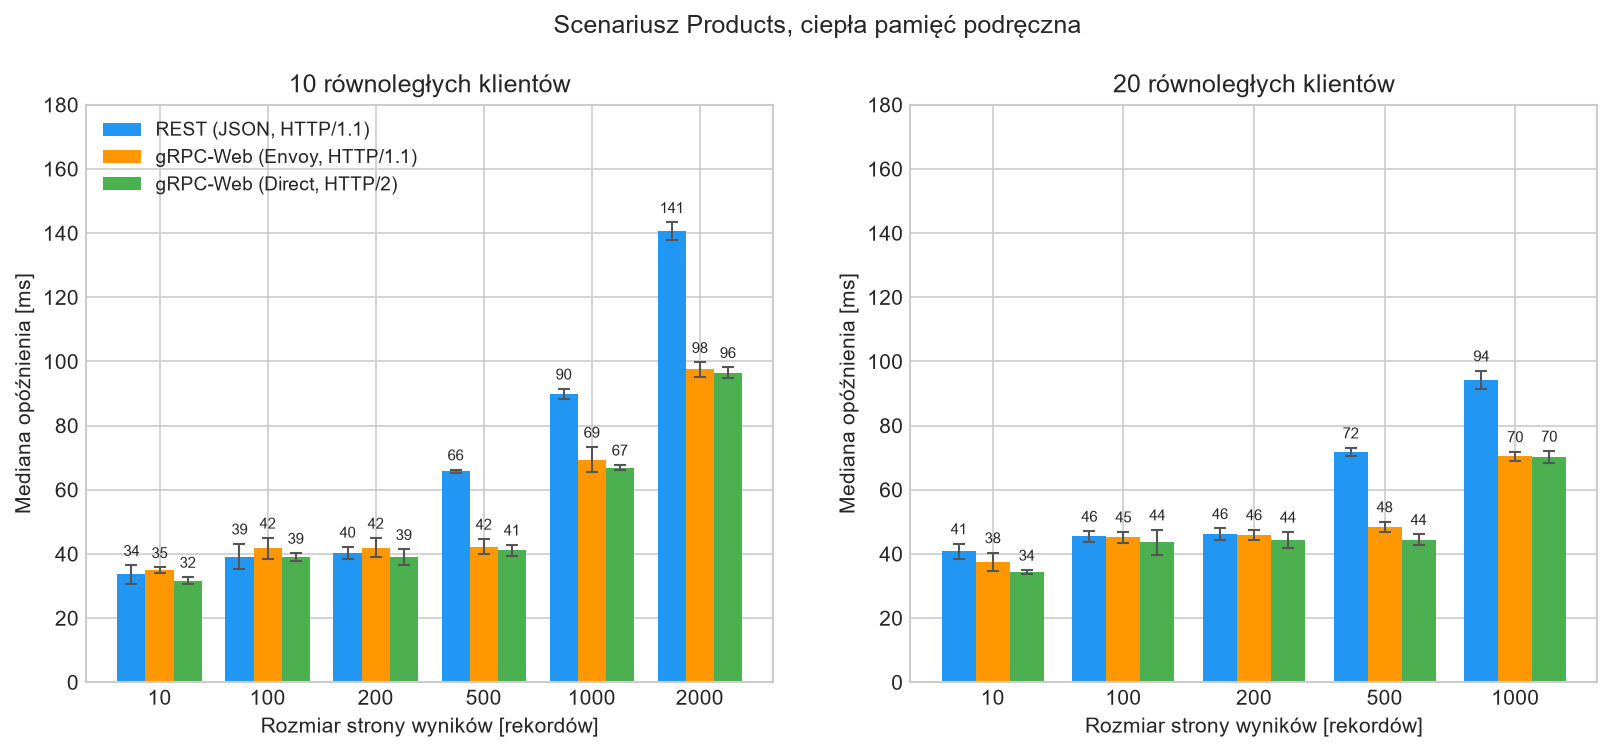
\includegraphics[width=\textwidth]{figures/chart_browser_products.png}
\caption{Mediana opóźnienia w~scenariuszach Products z~ciepłą pamięcią podręczną, dla dziesięciu i~dwudziestu równoległych klientów; słupki błędu odpowiadają 95\% przedziałowi ufności wartości centralnej.}
\label{fig:WykresProducts}
\end{figure}

Obraz uzyskany w~scenariuszu Echo przenosi się na~realną ścieżkę odczytu bez istotnych zmian, co~ilustruje rysunek~\ref{fig:WykresProducts}. Do~200~produktów na~stronę różnice mieszczą się w~przedziale od~jednego do~szesnastu procent, natomiast od~500~produktów przewaga wariantów binarnych stabilizuje się na~poziomie 26--38\%. Zgodność z~przewidywaniami modelu (tabela~\ref{tab:WeryfikacjaModelu}) jest w~tej grupie równie dobra jak w~scenariuszu Echo.

Scenariusz Products obejmuje wszystkie składniki obecne w~docelowym zastosowaniu: dostęp do~pamięci podręcznej, serializację po~stronie serwera, transmisję, deserializację w~silniku JavaScript oraz aktualizację drzewa dokumentu. Utrzymanie się przewagi w~tych warunkach wyklucza jej wyjaśnienie uproszczeniem scenariusza Echo.

Pomiar przy dwudziestu klientach daje ten~sam obraz relacji przy systematycznie wyższych wartościach bezwzględnych. Powtarzalność wyników w~tej grupie jest wysoka: współczynnik zmienności nie przekracza ośmiu procent. Najwyższa zmienność występuje przy najmniejszych ładunkach, gdzie mierzona wartość jest zdominowana przez opóźnienie propagacji i~podlega wahaniom warunków sieciowych w~większym stopniu względnym.

\subsection{Odczyt z~wymuszonym pominięciem pamięci podręcznej (PostgreSQL)}
\label{subsec:ProductsCold}

Wyniki uzyskane przy wymuszonym pominięciu bufora zestawia tabela~\ref{tab:ProductsCold}.

\begin{table}[htb]
\centering
\footnotesize
\caption{Mediana opóźnienia w~scenariuszach Products, wymuszone pominięcie pamięci podręcznej (PostgreSQL) [ms]; w~nawiasach współczynnik zmienności.}
\label{tab:ProductsCold}
\begin{tabular}{|c|c|c|c|c|}
\hline
\textbf{VU} & \textbf{PageSize} & \textbf{REST} & \textbf{Envoy} & \textbf{Direct} \\
\hline
10 & 10   & 36,8 (51,3\%) & 38,5 (46,7\%) & 36,7 (41,4\%) \\
10 & 100  & 84,9 (25,7\%) & 83,8 (24,4\%) & 80,1 (28,5\%) \\
10 & 200  & 82,8 (27,0\%) & 47,6 (40,9\%) & 89,9 (4,7\%) \\
10 & 500  & 76,7 (14,2\%) & 55,6 (33,5\%) & 75,6 (33,2\%) \\
10 & 1000 & 100,5 (4,6\%) & 91,9 (3,5\%) & 90,0 (11,0\%) \\
10 & 2000 & 187,5 (13,5\%) & 111,3 (7,7\%) & 116,0 (6,2\%) \\
\hline
20 & 500  & 89,1 (10,0\%) & 62,4 (30,9\%) & 78,3 (21,6\%) \\
20 & 1000 & 106,3 (8,9\%) & 109,2 (10,8\%) & 111,3 (17,7\%) \\
\hline
\end{tabular}
\end{table}

\begin{figure}[htb]
\centering
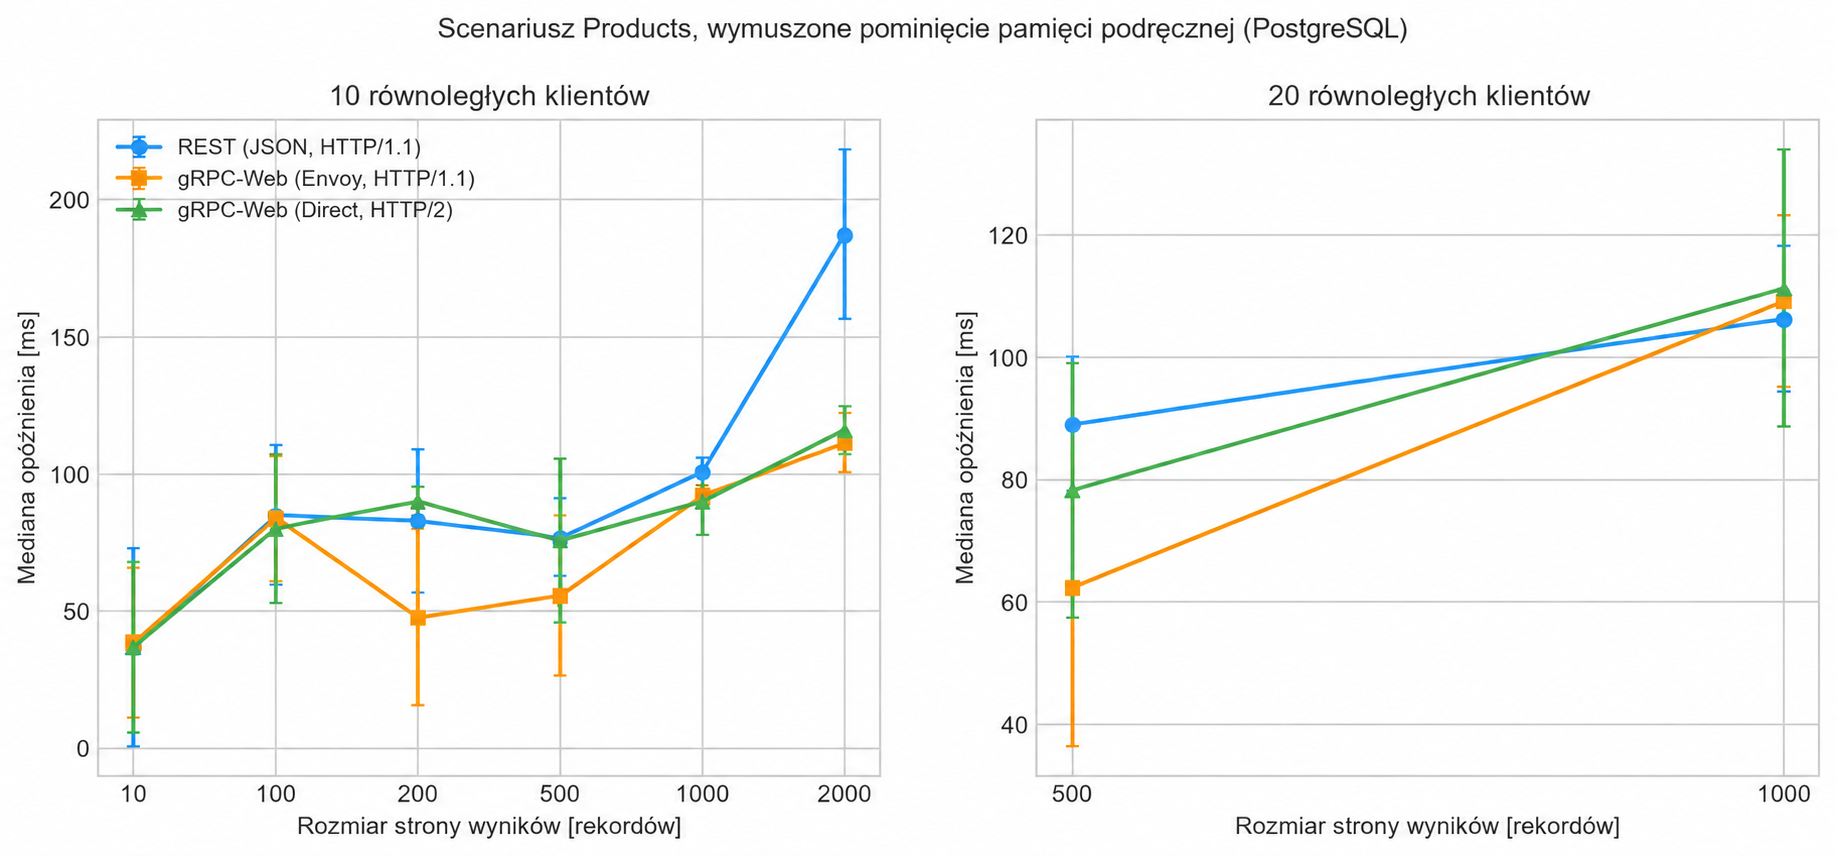
\includegraphics[width=\textwidth]{figures/chart_browser_products_cold.png}
\caption{Mediana opóźnienia w~scenariuszach Products z~wymuszonym pominięciem pamięci podręcznej (PostgreSQL); słupki błędu odpowiadają 95\% przedziałowi ufności wartości centralnej}
\label{fig:WykresProductsCold}
\end{figure}

Wymuszenie zapytania do~bazy danych przy każdym żądaniu wydłuża opóźnienie, a~przede wszystkim zwiększa jego zmienność: współczynnik zmienności osiąga w~skrajnych przypadkach 51\%, wobec kilku procent w~scenariuszach z~ciepłą pamięcią podręczną. W~konsekwencji przy małych stronach wyników kolejność protokołów jest niestabilna: w~konfiguracji o~200~produktach zmierzone mediany wynoszą 82,8, 47,6 i~89,9~ms, a~uporządkowanie to~nie powtarza się w~konfiguracji o~10~produktach. Różnice te~mieszczą się w~granicach zmienności tej grupy i~nie pozwalają wskazać szybszego protokołu. Zależność tę~wraz z~przedziałami ufności wartości centralnej przedstawia rysunek~\ref{fig:WykresProductsCold}.

Dla dużych stron wyników przewaga wariantów binarnych przewyższa poziom szumu: przy 2000~produktach REST osiąga 187,5~ms, wariant z~proxy 111,3~ms, a~wariant bezpośredni 116,0~ms, przy współczynniku zmienności nieprzekraczającym 13,5\%.

W~zakresie małych ładunków zmienność warstwy danych przewyższa różnicę wynikającą z~protokołu, więc ta~grupa scenariuszy nie służy do~porównywania protokołów. Ich wpływ izoluje scenariusz Echo, a~zachowanie w~warunkach realnych opisuje odczyt z~ciepłą pamięcią podręczną.

% -----------------------------------------------------------------------
\section{Analiza wydajności zapisu (Orders)}
\label{sec:AnalizaOrders}
% -----------------------------------------------------------------------

Scenariusze Orders angażują pełen łańcuch transakcyjny: walidację oraz zapis encji zamówienia wraz z~pozycjami. Zmierzone mediany opóźnienia przedstawia tabela~\ref{tab:OrdersLatency}.

\begin{table}[htb]
\centering
\footnotesize
\caption{Mediana opóźnienia w~scenariuszach Orders [ms]; w~nawiasach współczynnik zmienności}
\label{tab:OrdersLatency}
\begin{tabular}{|c|c|c|c|c|}
\hline
\textbf{VU} & \textbf{Pozycji} & \textbf{REST} & \textbf{Envoy} & \textbf{Direct} \\
\hline
10 & 1   & 85,4 (29,9\%) & 40,6 (50,7\%) & 35,6 (54,8\%) \\
10 & 10  & 94,2 (3,5\%)  & 89,1 (29,9\%) & 89,6 (40,3\%) \\
10 & 50  & 94,5 (2,5\%)  & 96,1 (0,7\%)  & 91,8 (22,0\%) \\
10 & 200 & 203,4 (39,1\%) & 225,9 (32,3\%) & 237,8 (32,1\%) \\
\hline
20 & 1   & 79,3 (39,8\%) & 43,8 (40,1\%) & 43,1 (47,9\%) \\
20 & 10  & 83,5 (35,0\%) & 89,9 (26,7\%) & 89,7 (4,9\%) \\
20 & 50  & 106,2 (40,0\%) & 101,2 (6,9\%) & 165,8 (21,6\%) \\
20 & 200 & 384,9 (16,6\%) & 334,7 (28,3\%) & 268,2 (28,4\%) \\
\hline
\end{tabular}
\end{table}

\begin{figure}[htb]
\centering
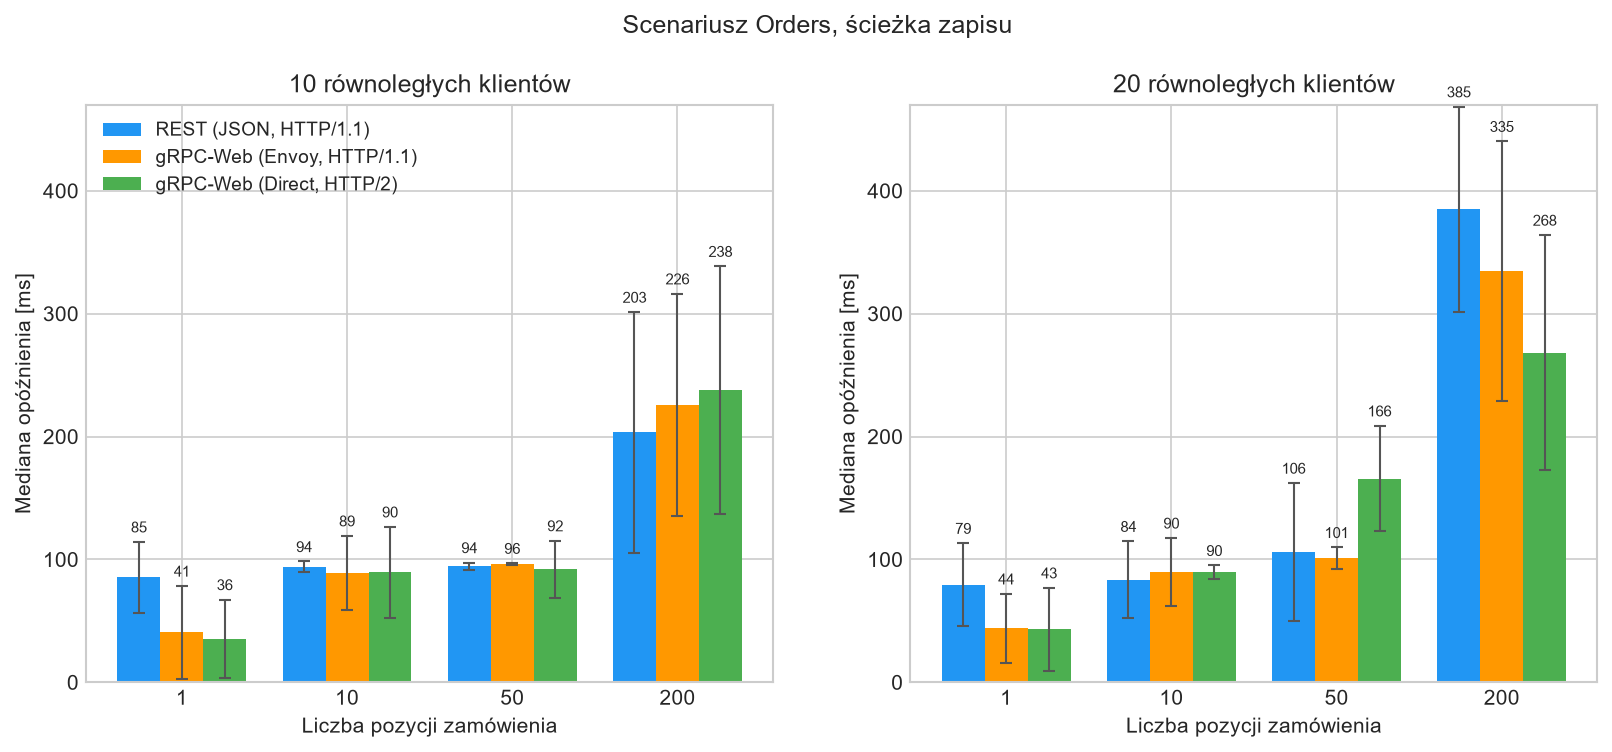
\includegraphics[width=\textwidth]{figures/chart_browser_orders.png}
\caption{Mediana opóźnienia w~scenariuszach Orders względem liczby pozycji zamówienia; słupki błędu odpowiadają 95\% przedziałowi ufności wartości centralnej}
\label{fig:WykresOrders}
\end{figure}

Scenariusze zapisu nie wykazują spójnej różnicy pomiędzy protokołami. Przy dziesięciu i~pięćdziesięciu pozycjach zamówienia mediany mieszczą się w~przedziale 83,5--165,8~ms. Górna wartość dotyczy wariantu Direct przy pięćdziesięciu pozycjach i~dwudziestu klientach; pozostałe mediany w~tej grupie wynoszą 83,5--106,2~ms. Przy dwustu pozycjach kolejność jest odmienna dla dwóch badanych poziomów obciążenia, a~współczynniki zmienności sięgają czterdziestu procent. Zestawienie median wraz z~przedziałami ufności wartości centralnej przedstawia rysunek~\ref{fig:WykresOrders}.

Wyjaśnienie wynika bezpośrednio z~modelu przedstawionego w~sekcji~\ref{sec:ModelOkna} oraz z~charakteru ścieżki zapisu. Żądania w~tym scenariuszu są~niewielkie: nawet dwieście pozycji zamówienia to~około siedemnastu kilobajtów, czyli znacznie mniej niż efektywny próg transmisji. Liczba obiegów pakietu pozostaje identyczna dla wszystkich formatów, a~mechanizm dający przewagę w~odczycie nie ma~tu~zastosowania. Jednocześnie czas odpowiedzi zdominowany jest przez stały koszt serwerowy: transakcję bazodanową obejmującą zapis encji.

W~badanych scenariuszach zapisu nie uzyskano stałej przewagi jednego wariantu. Szerokie przedziały ufności ograniczają rozstrzygalność różnic; wynik ten nie dowodzi równoważności protokołów ani braku wpływu sposobu komunikacji na~czas operacji.

% -----------------------------------------------------------------------
\section{Porównanie konfiguracji komunikacyjnych}
\label{sec:Dekompozycja}
% -----------------------------------------------------------------------

Ścieżka bezpośrednia korzysta z~HTTP/2 i~TLS, a~badany wariant REST z~HTTP/1.1. Wariant z~Envoy przenosi ładunek binarny, używając HTTP/1.1 na~odcinku pomiędzy przeglądarką a~proxy. Różnica REST--Envoy obejmuje obecność proxy i~odmienny sposób obsługi komunikatów. Różnica Envoy--Direct obejmuje jednocześnie pominięcie proxy, TLS oraz zmianę wersji HTTP. Zestawienie nie wyodrębnia przyczynowego udziału każdego z~tych czynników.

\begin{table}[htb]
\centering
\footnotesize
\caption{Czasy konfiguracji i~różnice względem mediany REST}
\label{tab:Dekompozycja}
\begin{tabular}{|l|c|c|c|c|c|}
\hline
\textbf{Konfiguracja} & \textbf{REST} & \textbf{Envoy} & \textbf{Direct} & $\frac{\mathrm{Envoy}-\mathrm{REST}}{\mathrm{REST}}$ & $\frac{\mathrm{Direct}-\mathrm{Envoy}}{\mathrm{REST}}$ \\
\hline
Echo, 2000 rek., VU=10      & 167,6 & 120,8 & 117,4 & $-$28\% & $-$2\% \\
Products, PS=500, VU=10     & 65,8  & 42,3  & 41,1  & $-$36\% & $-$2\% \\
Products, PS=1000, VU=10    & 89,9  & 69,4  & 66,9  & $-$23\% & $-$3\% \\
Products, PS=2000, VU=10    & 140,6 & 97,5  & 96,5  & $-$31\% & $-$1\% \\
Products, PS=500, VU=20     & 71,8  & 48,4  & 44,4  & $-$33\% & $-$6\% \\
\hline
\end{tabular}
\end{table}

\begin{figure}[htb]
\centering
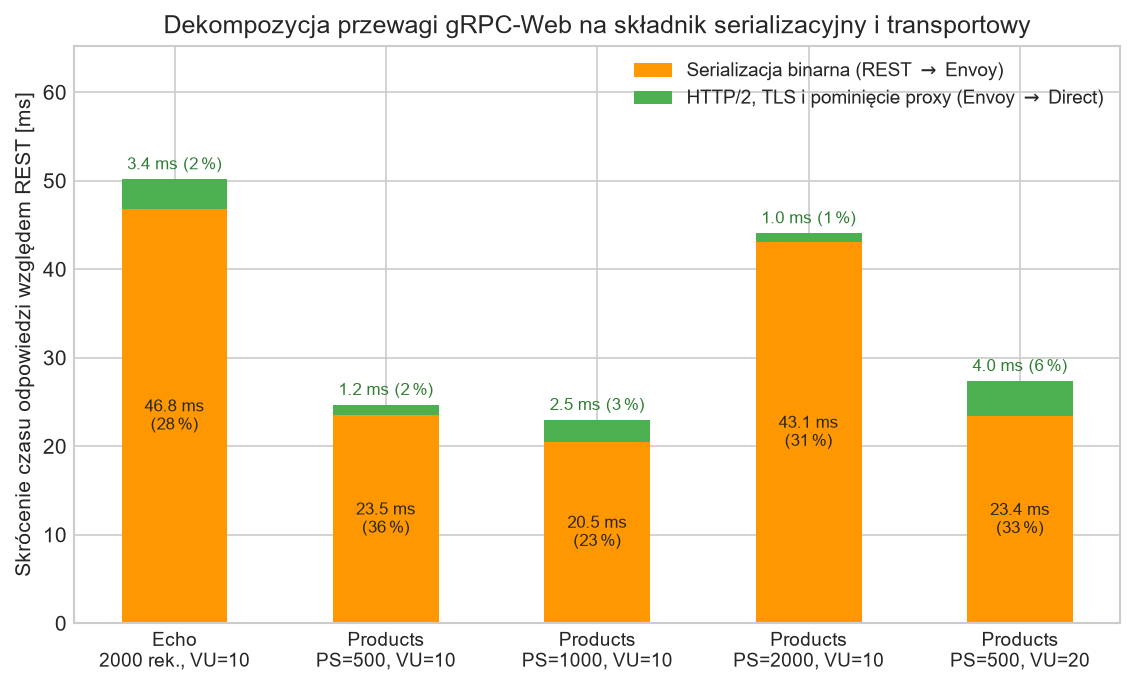
\includegraphics[width=0.7\textwidth]{figures/chart_browser_dekompozycja.png}
\caption{Różnice czasów trzech konfiguracji względem mediany opóźnienia REST; wartości procentowe odniesiono do~mediany REST}
\label{fig:WykresDekompozycja}
\end{figure}

Zestawienie w~postaci graficznej przedstawia rysunek~\ref{fig:WykresDekompozycja}. Obie kolumny procentowe odniesiono do~mediany REST, aby zachować wspólny mianownik, udział wariantu bezpośredniego względem samego Envoy podano przy weryfikacji hipotezy H5. W~konfiguracji Products, PS=500 i~VU=10 różnica REST--Direct wynosi 24,7~ms. Z~tej wartości 23,5~ms stanowi różnicę REST--Envoy, a~1,2~ms różnicę Envoy--Direct. Różnica REST--Envoy odpowiada zatem około 95\% całkowitej różnicy REST--Direct w~tej konfiguracji. Udział ten policzony dla wszystkich pięciu zestawień z~tabeli~\ref{tab:Dekompozycja} mieści się w~przedziale od~85\% (Products, PS=500, VU=20) do~98\% (Products, PS=2000, VU=10), natomiast różnica między wariantami Envoy i~Direct pozostaje znacznie mniejsza.

% -----------------------------------------------------------------------
\section{Skalowanie z~liczbą klientów i~granica stanowiska pomiarowego}
\label{sec:GranicaNarzedzia}
% -----------------------------------------------------------------------

Zakres badanych poziomów obciążenia wyznaczono na~podstawie odrębnego pomiaru, którego celem było ustalenie, do~jakiej liczby równoległych klientów stanowisko pomiarowe pozostaje wiarygodne. W~pomiarze tym zachowano stały, podstawowy czas namysłu, wobec czego przepustowość jest porównywalna pomiędzy poziomami obciążenia, adaptacyjny mechanizm opisany w~sekcji~\ref{subsec:BudzetPasma} obowiązuje w~macierzy właściwej. Wyniki dla konfiguracji o~100~produktach na~stronę i~ciepłej pamięci podręcznej przedstawia tabela~\ref{tab:Skalowanie}.

\begin{table}[htb]
\centering
\footnotesize
\caption{Skalowanie z~liczbą równoległych klientów: mediana opóźnienia [ms] i~przepustowość [operacji/s]}
\label{tab:Skalowanie}
\begin{tabular}{|c|c|c|c|c|c|c|}
\hline
\textbf{VU} & \multicolumn{3}{c|}{\textbf{Mediana opóźnienia [ms]}} & \multicolumn{3}{c|}{\textbf{Przepustowość [oper./s]}} \\
\hline
 & \textbf{REST} & \textbf{Envoy} & \textbf{Direct} & \textbf{REST} & \textbf{Envoy} & \textbf{Direct} \\
\hline
10 & 38,1  & 41,4  & 39,5  & 40,7 & 40,7 & 38,3 \\
20 & 50,9  & 50,0  & 44,5  & 40,8 & 58,7 & 59,3 \\
30 & 64,8  & 61,8  & 54,9  & 72,3 & 69,9 & 68,3 \\
50 & 140,3 & 122,5 & 113,2 & 75,4 & 63,8 & 64,6 \\
\hline
\end{tabular}
\end{table}

\begin{figure}[htb]
\centering
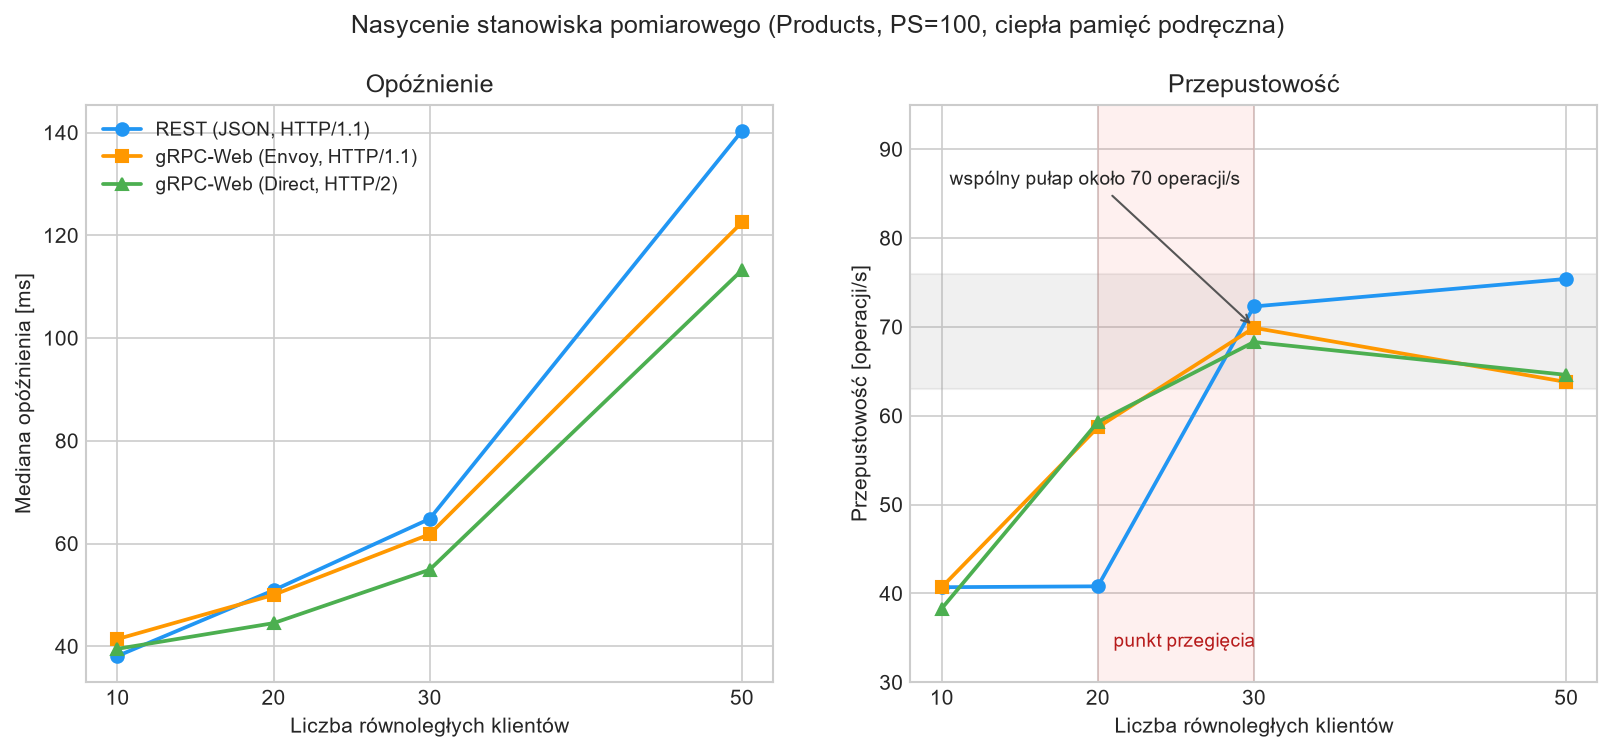
\includegraphics[width=\textwidth]{figures/chart_browser_nasycenie.png}
\caption{Opóźnienie i~przepustowość względem liczby równoległych klientów; szary pas oznacza wspólny pułap przepustowości, a~różowy położenie punktu przegięcia}
\label{fig:WykresNasycenie}
\end{figure}

Zestawienie, zilustrowane na~rysunku~\ref{fig:WykresNasycenie}, ujawnia obraz nasycenia. Oba warianty gRPC-Web osiągają maksimum przepustowości przy trzydziestu klientach, na~poziomie około siedemdziesięciu operacji na~sekundę, po~czym przy pięćdziesięciu klientach wartość ta~spada. W~ścieżce REST przepustowość rośnie w~tym zakresie wolniej i~przy pięćdziesięciu klientach osiąga 75,4~operacji na~sekundę, pozostając w~tym samym rzędzie wielkości. Opóźnienie narasta przy tym monotonicznie, z~38 do~140~ms. Powyżej punktu przegięcia zwiększanie współbieżności wydłuża wyłącznie czas oczekiwania w~kolejce, bez korzyści przepustowościowej.

W~odczycie z~ciepłą pamięcią podręczną REST zwraca gotowy dokument JSON z~Redis, a~oba warianty gRPC odtwarzają obiekt z~bajtów Protocol Buffers i~ponownie go~serializują. Zbliżony pułap przepustowości mimo tych różnic jest przesłanką ograniczenia po~stronie wspólnego klienta pomiarowego, na~przykład rywalizacji o~zasoby pomiędzy kontekstami przeglądarki. Jednoznaczne wskazanie miejsca ograniczenia byłoby możliwe dopiero po~zestawieniu tych pomiarów z~metrykami serwerowymi, ponieważ samo porównanie ścieżek dopuszcza również wspólne ograniczenie po~stronie serwera lub sieci.

Wniosek ten stanowił podstawę ograniczenia macierzy badawczej do~dziesięciu i~dwudziestu klientów, to~jest poniżej punktu przegięcia. Przyjęto zasadę, że~węższy zakres współbieżności z~wynikami wiarygodnymi jest wartościowszy niż zakres szerszy z~wynikami opisującymi ograniczenia narzędzia.

% -----------------------------------------------------------------------
\section{Powtarzalność pomiarów i~przedziały ufności}
\label{sec:Zmiennosc}
% -----------------------------------------------------------------------

Pięciokrotne wykonanie całej macierzy umożliwia ocenę powtarzalności. Tabela~\ref{tab:Zmiennosc} przedstawia rozkład współczynnika zmienności median przebiegów w~poszczególnych grupach scenariuszy.

\begin{table}[htb]
\centering
\footnotesize
\caption{Współczynnik zmienności median pięciu przebiegów, w~podziale na~grupy scenariuszy}
\label{tab:Zmiennosc}
\begin{tabular}{|l|c|c|c|}
\hline
\textbf{Grupa scenariuszy} & \textbf{Minimum} & \textbf{Typowo} & \textbf{Maksimum} \\
\hline
Echo                          & 0,7\% & 1,5--5\% & 11,5\% \\
Products, ciepła pamięć       & 0,6\% & 2--6\%   & 8,0\% \\
Products, pominięcie pamięci  & 3,5\% & 10--30\% & 51,3\% \\
Orders                        & 0,7\% & 20--40\% & 54,8\% \\
\hline
\end{tabular}
\end{table}

Rozrzut wyników rośnie wraz z~udziałem warstwy danych w~czasie
odpowiedzi. Najwyższą powtarzalność wykazują scenariusze
Echo, nieodwołujące się do~bazy ani pamięci podręcznej oraz scenariusze
odczytu z~ciepłą pamięcią podręczną. Scenariusze wymuszające zapytanie do~bazy
oraz scenariusze zapisu charakteryzują się zmiennością o~rząd wielkości
wyższą, ponieważ angażują mechanizmy trwałego utrwalania danych, dziennik
transakcji oraz blokady wierszy.

% -----------------------------------------------------------------------
\subsection{Przedziały ufności i~rozstrzygalność zmierzonych różnic}
\label{subsec:WynikiPrzedzialy}
% -----------------------------------------------------------------------

Zestawienia przedstawione w~poprzednich sekcjach podają wartości centralne wraz z~miarą rozrzutu. Ocena, czy zaobserwowana różnica jest rzeczywista, wymaga miary niepewności samej wartości centralnej. Przedziały ufności wyznaczone dla wartości centralnej według równania~\ref{eq:PrzedzialUfnosci} zestawia tabela~\ref{tab:PrzedzialyCentralne}.

\begin{table}[htb]
\centering
\footnotesize
\caption{Przedziały ufności 95\% dla wartości centralnej opóźnienia [ms]; $k=5$ przebiegów, $t=2{,}776$}
\label{tab:PrzedzialyCentralne}
\begin{tabular}{|l|c|c|c|}
\hline
\textbf{Konfiguracja} & \textbf{REST} & \textbf{Envoy} & \textbf{Direct} \\
\hline
Echo, 200 rek., VU=10      & 32,5 $\pm$ 0,4 & 33,4 $\pm$ 0,6 & 31,4 $\pm$ 0,5 \\
Echo, 500 rek., VU=10      & 59,7 $\pm$ 0,8 & 35,2 $\pm$ 0,8 & 34,0 $\pm$ 1,0 \\
Echo, 2000 rek., VU=10     & 168,0 $\pm$ 1,5 & 120,4 $\pm$ 2,7 & 117,5 $\pm$ 2,4 \\
Echo, 500 rek., VU=20      & 60,6 $\pm$ 1,3 & 39,7 $\pm$ 3,0 & 37,0 $\pm$ 5,3 \\
\hline
Products, PS=200, VU=10    & 40,6 $\pm$ 1,9 & 42,0 $\pm$ 3,0 & 39,2 $\pm$ 2,4 \\
Products, PS=500, VU=10    & 65,8 $\pm$ 0,5 & 42,3 $\pm$ 2,4 & 40,8 $\pm$ 1,8 \\
Products, PS=1000, VU=10   & 90,0 $\pm$ 1,5 & 69,9 $\pm$ 3,9 & 66,9 $\pm$ 0,8 \\
Products, PS=2000, VU=10   & 140,8 $\pm$ 2,7 & 97,5 $\pm$ 2,2 & 96,8 $\pm$ 1,6 \\
Products, PS=500, VU=20    & 71,9 $\pm$ 1,3 & 48,7 $\pm$ 1,7 & 44,4 $\pm$ 1,7 \\
Products, PS=1000, VU=20   & 94,8 $\pm$ 2,8 & 70,7 $\pm$ 1,4 & 70,3 $\pm$ 1,9 \\
\hline
Orders, 10 poz., VU=10     & 93,2 $\pm$ 4,1 & 81,3 $\pm$ 30,2 & 73,7 $\pm$ 36,9 \\
Orders, 50 poz., VU=10     & 93,5 $\pm$ 3,0 & 96,0 $\pm$ 0,8 & 86,2 $\pm$ 23,5 \\
Orders, 10 poz., VU=20     & 72,0 $\pm$ 31,3 & 83,0 $\pm$ 27,5 & 89,1 $\pm$ 5,4 \\
Orders, 50 poz., VU=20     & 112,7 $\pm$ 55,9 & 101,2 $\pm$ 8,6 & 160,3 $\pm$ 43,0 \\
\hline
\end{tabular}
\end{table}

Wartością centralną jest tutaj średnia median pięciu przebiegów, zgodnie z~jednostką analizy przyjętą w~sekcji~\ref{subsec:MetodykaPrzedzialow}, podczas gdy tabele w~poprzednich sekcjach podają medianę wyznaczoną ze~wszystkich pomiarów łącznie. W~grupach o~niskim rozrzucie obie statystyki są~praktycznie zbieżne, w~scenariuszach zapisu rozchodzą się wyraźnie, ponieważ rozkład czasów jest tam silnie skośny.

W~scenariuszach Echo oraz w~odczycie z~ciepłą pamięcią podręczną połówkowa szerokość przedziału nie przekracza kilku milisekund, natomiast w~scenariuszach zapisu sięga kilkudziesięciu, przekraczając w~skrajnym przypadku połowę samej wartości centralnej.

Zasadnicze znaczenie ma~jednak zestawienie różnic pomiędzy protokołami w~układzie sparowanym, przedstawione w~tabeli~\ref{tab:PrzedzialyRoznic}. Wartość dodatnia oznacza, że~pierwszy z~wymienionych protokołów jest wolniejszy. Kolejne akapity omawiają wyniki dla dużych i~małych odpowiedzi, wariantów gRPC-Web oraz scenariuszy zapisu.

\begin{table}[htb]
\centering
\footnotesize
\caption{Przedziały ufności 95\% dla różnic sparowanych w~obrębie przebiegu [ms]; wartość dodatnia oznacza dłuższy czas odpowiedzi pierwszego z~protokołów}
\label{tab:PrzedzialyRoznic}
\begin{tabular}{|l|c|c|c|c|}
\hline
\textbf{Konfiguracja} & \textbf{REST--Envoy} & \textbf{REST--Direct} & \textbf{Envoy--Direct} & \textbf{Rozstrz.} \\
\hline
Echo, 200 rek., VU=10      & $-$0,9 $\pm$ 0,9 & 1,1 $\pm$ 0,7 & 2,0 $\pm$ 0,3 & tak \\
Echo, 500 rek., VU=10      & 24,5 $\pm$ 1,0 & 25,8 $\pm$ 1,6 & 1,2 $\pm$ 0,9 & tak \\
Echo, 2000 rek., VU=10     & 47,6 $\pm$ 3,8 & 50,5 $\pm$ 3,3 & 2,9 $\pm$ 3,4 & tak \\
Echo, 500 rek., VU=20      & 20,9 $\pm$ 2,7 & 23,6 $\pm$ 5,7 & 2,7 $\pm$ 7,2 & tak \\
\hline
Products, PS=200, VU=10    & $-$1,4 $\pm$ 3,8 & 1,4 $\pm$ 2,5 & 2,7 $\pm$ 2,4 & nie \\
Products, PS=500, VU=10    & 23,4 $\pm$ 2,4 & 24,9 $\pm$ 1,6 & 1,5 $\pm$ 1,4 & tak \\
Products, PS=1000, VU=10   & 20,1 $\pm$ 4,3 & 23,1 $\pm$ 1,2 & 3,0 $\pm$ 3,7 & tak \\
Products, PS=2000, VU=10   & 43,3 $\pm$ 4,9 & 44,0 $\pm$ 3,5 & 0,8 $\pm$ 2,2 & tak \\
Products, PS=500, VU=20    & 23,2 $\pm$ 1,4 & 27,4 $\pm$ 1,5 & 4,2 $\pm$ 1,8 & tak \\
Products, PS=1000, VU=20   & 24,1 $\pm$ 3,6 & 24,5 $\pm$ 1,9 & 0,4 $\pm$ 3,1 & tak \\
\hline
Orders, 10 poz., VU=10     & 12,0 $\pm$ 32,5 & 19,5 $\pm$ 35,5 & 7,6 $\pm$ 31,9 & nie \\
Orders, 50 poz., VU=10     & $-$2,4 $\pm$ 3,1 & 7,4 $\pm$ 25,4 & 9,8 $\pm$ 23,8 & nie \\
Orders, 10 poz., VU=20     & $-$11,0 $\pm$ 21,3 & $-$17,1 $\pm$ 28,9 & $-$6,1 $\pm$ 22,6 & nie \\
Orders, 50 poz., VU=20     & 11,5 $\pm$ 60,1 & $-$47,6 $\pm$ 76,0 & $-$59,1 $\pm$ 45,2 & nie \\
\hline
\multicolumn{5}{|l|}{\footnotesize Kolumna \textit{Rozstrz.} odnosi się do~różnicy REST--Direct} \\
\hline
\end{tabular}
\end{table}

W~każdej konfiguracji odczytu od~500~rekordów przewaga wariantów binarnych jest rozstrzygnięta z~dużym marginesem: przedział dla różnicy REST--Direct wynosi na~przykład $24{,}9 \pm 1{,}6$~ms przy 500~produktach oraz $50{,}5 \pm 3{,}3$~ms przy 2000~rekordach scenariusza Echo.

W~zakresie małych ładunków obraz jest bardziej złożony, niż wskazywałaby sama wielkość różnicy. W~scenariuszu Products przy 200~produktach różnica REST--Direct wynosi $1{,}4 \pm 2{,}5$~ms, więc nie jest rozstrzygnięta. W~scenariuszu Echo przy tej~samej liczbie rekordów różnica wynosi $1{,}1 \pm 0{,}7$~ms i~pozostaje bez znaczenia praktycznego wobec opóźnienia obiegu pakietu wynoszącego 26,2~ms.

Różnica pomiędzy oboma wariantami gRPC-Web jest rozstrzygnięta jedynie w~pięciu z~dziesięciu konfiguracji odczytu, a~jej wielkość mieści się w~przedziale od~$0{,}4 \pm 3{,}1$ do~$4{,}2 \pm 1{,}8$~ms. Wielkość efektu jest zatem porównywalna z~niepewnością jego oszacowania, co~uzasadnia wniosek o~drugorzędnym znaczeniu wyboru pomiędzy wariantem bezpośrednim a~wariantem z~proxy.

W~scenariuszach zapisu żadna z~różnic REST--Direct nie jest rozstrzygnięta. Przedziały są~w~tej grupie od~kilku do~kilkudziesięciu razy szersze niż w~odczycie. Dla pozostałych porównań jedyny wyjątek dotyczy pary Envoy--Direct przy pięćdziesięciu pozycjach i~dwudziestu klientach ($-59{,}1 \pm 45{,}2$~ms). Znak tej różnicy jest jednak przeciwny niż w~pozostałych komórkach tej grupy, a~jej wartość wynika z~jednego odstającego przebiegu.

% -----------------------------------------------------------------------
\section{Weryfikacja hipotez badawczych}
\label{sec:WeryfikacjaHipotez}
% -----------------------------------------------------------------------

\begin{sloppypar}
\textbf{H1 (warianty gRPC-Web osiągają niższe opóźnienie niż REST, a~przewaga rośnie z~rozmiarem odpowiedzi):} wyniki częściowo wspierają hipotezę. Przewaga występuje i~jest znaczna: 26--43\% przy odpowiedziach od~500~rekordów. Wzrost nie ma~charakteru ciągłego, dlatego wyniki nie potwierdzają monotonicznego wzrostu przewagi wraz z~rozmiarem odpowiedzi. Efekt ujawnia się po~przekroczeniu efektywnego progu transmisji, natomiast w~zakresie do~200~rekordów pozostaje w~granicach kilku procent.
\end{sloppypar}

\begin{sloppypar}
\textbf{H2 (przy małych odpowiedziach różnice pozostają małe w~wartościach bezwzględnych):} hipoteza uzyskała wsparcie w~badanych konfiguracjach. Przy odpowiedziach do~200~rekordów różnice wynoszą od~jednego do~szesnastu procent, przy wartościach bezwzględnych rzędu kilku milisekund, wobec opóźnienia obiegu pakietu wynoszącego 26,2~ms. Samo opóźnienie propagacji stanowi w~tym zakresie od~około pięćdziesięciu
siedmiu procent czasu odpowiedzi przy dwudziestu równoległych klientach
i~dwustu rekordach do~siedemdziesięciu ośmiu procent przy dziesięciu
klientach i~dziesięciu rekordach. Nie przyjęto z~góry progu istotności praktycznej; wielkość różnic w~tym zakresie oceniono na~tle dominującego udziału opóźnienia propagacji.
\end{sloppypar}

\begin{sloppypar}
\textbf{H3 (wariant gRPC-Web przez Envoy zachowuje przewagę względem REST przy HTTP/1.1 na~odcinku przeglądarkowym):} wyniki częściowo potwierdzają hipotezę. W~konfiguracjach z~większymi odpowiedziami wariant przez Envoy uzyskuje przewagę nad REST, dla małych odpowiedzi relacja nie jest równie wyraźna. W~konfiguracji Products, PS=500 i~VU=10 różnica REST--Envoy stanowi około 95\% różnicy REST--Direct. Układ eksperymentalny nie pozwala przypisać tej różnicy pojedynczemu czynnikowi, co~omówiono w~sekcji~\ref{sec:Dekompozycja}.
\end{sloppypar}

\begin{sloppypar}
\textbf{H4 (w~operacjach zapisu różnice zanikają):} hipoteza nierozstrzygnięta. Przy dziesięciu i~pięćdziesięciu pozycjach zamówienia mediany wynoszą 83,5--165,8~ms, a~przedziały ufności dla różnic REST--Direct obejmują zero, wyjątek dla pary Envoy--Direct omówiono w~sekcji~\ref{subsec:WynikiPrzedzialy}. Granice interpretacji tego wyniku przedstawiono przy analizie scenariuszy zapisu w~sekcji~\ref{sec:AnalizaOrders}.
\end{sloppypar}

\textbf{H5 (wariant Direct osiąga niższe opóźnienie niż wariant z~proxy Envoy):} wyniki częściowo wskazują na zgodność z hipotezą. Wariant bezpośredni ma~niższą medianę w~każdej konfiguracji odczytu z~ciepłą pamięcią podręczną oraz scenariusza Echo. Skrócenie czasu wynosi około 0,4--9,2\%. Nie wszystkie różnice są~jednak rozstrzygnięte statystycznie. W~grupie scenariuszy z~wymuszonym pominięciem pamięci podręcznej relacja ta~nie zachodzi konsekwentnie. Wybór wariantu wdrożenia wymaga uwzględnienia również topologii systemu.

% -----------------------------------------------------------------------
\section{Zestawienie wyników z~dotychczasowymi badaniami}
\label{sec:ZestawienieZBadaniami}
% -----------------------------------------------------------------------

Uzyskane wyniki odniesiono do~prac omówionych w~rozdziale~\ref{cha:StanBadan}. Zestawienie ma~charakter jakościowy, ponieważ przytaczane badania stosowały odmienne granice pomiaru, środowiska uruchomieniowe i~narzędzia obciążające, a~różnice w~tych warunkach wykluczają bezpośrednie porównywanie raportowanych wartości procentowych.

Śliwa i~Pańczyk~\cite{bib:SliwaPanczyk2021} odnotowali korzystne czasy odpowiedzi REST w~wielu scenariuszach przy jednoczesnym mniejszym wolumenie danych przesyłanych przez gRPC. Pomiary przedstawione w~niniejszej pracy potwierdzają drugą część tej obserwacji: serializacja binarna zmniejszyła wolumen o~42,8--43,4\% w~scenariuszu Products i~o~32,8--33,5\% w~scenariuszu Echo. Relacja czasów odpowiedzi zależała przy tym od~rozmiaru odpowiedzi. Do~200~rekordów różnice wynosiły od~jednego do~szesnastu procent, przy wartościach bezwzględnych rzędu kilku milisekund, a~przewaga wariantów binarnych rzędu 26--43\% ujawniła się dopiero przy odpowiedziach od~około 500~rekordów. Rozbieżność wobec cytowanej pracy wyjaśniają dwa czynniki: granica pomiaru, obejmująca w~niniejszym eksperymencie również dekodowanie odpowiedzi i~aktualizację drzewa dokumentu oraz opóźnienie obiegu pakietu wynoszące 26,2~ms, które w~zakresie małych odpowiedzi stanowiło od~pięćdziesięciu siedmiu do~siedemdziesięciu ośmiu procent czasu operacji. W~konfiguracjach, w~których odpowiedź pozostaje poniżej efektywnego progu transmisji, oba zestawy wyników pozostają zgodne.

Wynik Niswara i~współautorów~\cite{bib:Niswar2024}, wskazujący najkrótsze czasy odpowiedzi gRPC przy odczytach obsługiwanych z~pamięci podręcznej, zgadza się kierunkowo z~pomiarami scenariusza Products z~ciepłą pamięcią podręczną, w~którym oba warianty gRPC-Web osiągnęły niższe mediany od~REST. Skali tej przewagi nie można jednak przenosić między badaniami, ponieważ cytowana praca dotyczyła usług napisanych w~języku Go, obciążanych generatorem żądań, a~pomiar kończył się na~odpowiedzi usługi.

Spostrzeżenie Bolanowskiego i~współautorów~\cite{bib:Bolanowski2022} oraz Kamińskiego i~współautorów~\cite{bib:Kaminski2023} o~zależności wyniku od~rodzaju operacji i~konfiguracji transportu znajduje w~przedstawionych pomiarach bezpośrednie potwierdzenie. Kierunek relacji pomiędzy protokołami zmieniał się wraz ze~scenariuszem: w~odczycie dużych zbiorów przewaga wariantów binarnych była wyraźna, natomiast w~scenariuszach zapisu, gdzie czas wyznaczała transakcja bazodanowa, stałej przewagi nie zaobserwowano. Podobny wpływ miała konfiguracja warstwy transportowej: kompresja gzip zmniejszyła w~oszacowaniu przewagę objętościową formatu binarnego z~około 33\% do~15--18\%, co~zgodnie z~przedstawionym modelem przesuwałoby granicę rozmiaru odpowiedzi, przy której różnice czasowe pomiędzy wariantami stają się zauważalne.

Prace dotyczące GraphQL~\cite{bib:Brito2019,bib:Vadlamani2021,bib:Jin2025} wskazują na~wymóg, by~porównywane ścieżki zwracały ten~sam zakres informacji i~wykonywały tę~samą logikę biznesową. Eksperyment spełnia ten warunek: wszystkie trzy warianty korzystały ze~wspólnej aplikacji klienckiej, tych~samych danych oraz identycznej ścieżki prezentacji, a~pomiar kończył się w~tym~samym punkcie cyklu przetwarzania.

Przedstawione zestawienie wskazuje, że~uzyskane wyniki uzupełniają dotychczasowe ustalenia o~warunki, w~których obserwowana w~pomiarach interfejsów programistycznych przewaga formatu binarnego pozostaje odczuwalna w~aplikacji przeglądarkowej. Granicę tę~wyznacza w~badanym środowisku relacja rozmiaru odpowiedzi do~efektywnego progu transmisji, przy czym sam wybór protokołu pozostaje wobec niej czynnikiem wtórnym.

% -----------------------------------------------------------------------
\section{Rekomendacje i~wytyczne wdrożeniowe}
\label{sec:RekomendacjeArchitektoniczne}
% -----------------------------------------------------------------------

Uzyskane wyniki dostarczają mierzalnych kryteriów doboru mechanizmu komunikacji do~charakterystyki konkretnego systemu, bezwarunkowe zastąpienie REST przez gRPC-Web nie znajduje w~nich uzasadnienia. Decyzja powinna wynikać z~rozmiaru przesyłanych danych, parametrów łącza, dominującego rodzaju operacji oraz wymagań eksploatacyjnych.

\subsection{Rekomendacje architektoniczne}

\begin{enumerate}
    \item \textbf{Rozmiar odpowiedzi należy oceniać względem efektywnego progu transmisji.} Zastosowanie formatu binarnego przynosi istotną korzyść wtedy, gdy zmniejszenie wolumenu ogranicza liczbę wymian pakietów. W~badanym środowisku efekt pojawiał się przy nieskompresowanych odpowiedziach od~około 500~rekordów i~osiągał 26--43\%. Dla małych odpowiedzi różnice pozostawały na~poziomie pojedynczych milisekund, dlatego sam wybór gRPC-Web nie powinien być traktowany jako uniwersalna optymalizacja.

    \item \textbf{Przed zmianą protokołu należy zmierzyć ładunek po~kompresji.} Kompresja gzip zmniejszyła w~oszacowaniu przewagę objętościową Protocol Buffers z~około 33\% do~15--18\% i~sprowadziła wszystkie analizowane odpowiedzi poniżej efektywnego progu transmisji. W~systemach podających dokumenty JSON z~kompresją właściwym pierwszym krokiem jest pomiar rzeczywistego rozmiaru odpowiedzi, a~następnie test opóźnienia w~docelowej sieci. Jeżeli ładunek nadal przekracza efektywny próg transmisji, należy rozważyć również paginację, ograniczenie pól odpowiedzi lub zmianę sposobu agregacji danych.

    \item \textbf{Rodzaj operacji należy rozważyć przed formatem komunikatu.} W~odczycie dużych zbiorów koszt transmisji może dominować i~uzasadniać zastosowanie gRPC-Web. W~operacjach zapisu angażujących transakcję bazodanową różnice pomiędzy protokołami nie były rozstrzygalne, ponieważ czas odpowiedzi wyznaczała warstwa persystencji. W~takich ścieżkach priorytetem powinny być optymalizacja zapytań, zakres transakcji i~organizacja zapisu, natomiast protokół należy dobierać ze~względu na~kontrakt, interoperacyjność i~koszt utrzymania.

    \item \textbf{Wybór pomiędzy wariantem bezpośrednim a~proxy powinien wynikać z~topologii systemu.} W~scenariuszach Echo i~odczytu z~ciepłą pamięcią podręczną Direct skracał medianę czasu względem Envoy o~około 0,4--9,2\%, przy czym nie wszystkie różnice były rozstrzygnięte statystycznie. Obsługa bezpośrednia upraszcza ścieżkę żądania i~ogranicza liczbę komponentów, natomiast serwer pośredniczący może być uzasadniony, gdy architektura wymaga wspólnej warstwy routingu i~centralnej konfiguracji ruchu. Nie należy rezygnować z~proxy wyłącznie na~podstawie oczekiwania znaczącego skrócenia czasu odpowiedzi.

    \item \textbf{Pamięć podręczna powinna być traktowana również jako mechanizm stabilizacji czasu odpowiedzi.} W~scenariuszach z~ciepłą pamięcią podręczną współczynnik zmienności wynosił typowo 2--6\%, natomiast przy wymuszonym dostępie do~bazy wzrastał do~10--30\%, a~maksymalnie do~51,3\%. Cache-Aside skraca więc czas odpowiedzi i~jednocześnie zwiększa jego przewidywalność. Wymaga to~jednocześnie jawnej polityki unieważniania danych oraz osobnego monitorowania ścieżek trafienia i~chybienia.
\end{enumerate}

\subsection{Wytyczne wdrożeniowe}

\begin{enumerate}
    \item \textbf{Test wydajnościowy należy prowadzić w~warunkach odpowiadających docelowemu wdrożeniu.} Powinien on~obejmować rzeczywistą przeglądarkę, końcową konfigurację TLS, kompresji i~serwerów pośredniczących oraz reprezentatywne opóźnienie sieci. Pomiar wyłącznie wewnątrz centrum danych może ukryć efekt zależny od~liczby obiegów pakietu, natomiast test bez kompresji może zawyżyć przewagę formatu binarnego względem konfiguracji produkcyjnej.

    \item \textbf{Należy oddzielić ograniczenia systemu od~ograniczeń generatora obciążenia.} Wspólny pułap przepustowości wszystkich wariantów ujawnił punkt nasycenia stanowiska pomiarowego; wyniki sugerują udział ograniczenia po~stronie klienta, lecz nie pozwalają jednoznacznie zlokalizować wąskiego gardła. Przed interpretacją wyników trzeba więc wykonać pomiar skalowania i~wyznaczyć punkt przegięcia. Badania większej współbieżności powinny wykorzystywać wiele maszyn generujących ruch, przy zachowaniu pomiaru czasu wewnątrz strony i~kontroli obciążenia każdej z~nich.

    \item \textbf{Porównywane ścieżki muszą zachowywać symetrię funkcjonalną.} Powinny wykonywać tę~samą logikę biznesową, korzystać z~tych~samych danych i~kończyć pomiar w~tym~samym punkcie cyklu renderowania. Należy też pomiarowo potwierdzić negocjowaną wersję HTTP, liczbę połączeń, rozmiar odpowiedzi i~stan pamięci podręcznej. Bez tej kontroli zmierzona różnica może pochodzić z~odmiennej implementacji obu ścieżek.

    \item \textbf{Metryki serwerowe należy zestawiać z~pomiarem wykonanym po~stronie klienta.} Metryki serwerowe powinny obejmować co~najmniej czas obsługi żądania, liczbę żądań, wykorzystanie zasobów oraz zachowanie środowiska uruchomieniowego. Ich zestawienie z~czasem mierzonym w~przeglądarce pozwala rozróżnić koszt przetwarzania po~stronie usługi od~transmisji, deserializacji i~aktualizacji interfejsu.

    \item \textbf{Decyzję protokołową należy okresowo ponawiać po~zmianach systemu.} Zmiana modelu odpowiedzi, poziomu kompresji, lokalizacji użytkowników, konfiguracji proxy lub sposobu korzystania z~pamięci podręcznej może przesunąć granicę, przy której format binarny daje korzyść. Kryterium wdrożeniowym powinien być wynik powtarzalnego testu dla reprezentatywnych scenariuszy danego systemu, ważny w~warunkach, w~jakich go~uzyskano.
\end{enumerate}
